\documentclass[twocolumn,amsmath,amssymb]{revtex4}
%\documentclass[preprint,amsmath,amssymb]{revtex4}
\usepackage{graphicx}
\usepackage{color}
\usepackage{amsmath}
\newcommand{\pd}[0]{\partial}
\newcommand{\pr}[1]{#1^{\prime}}
\newcommand\given[1][]{\:#1\vert\:}
\newcommand*\diff{\mathop{}\!\mathrm{d}}
\newcommand*\Diff[1]{\mathop{}\!\mathrm{d^#1}}

\begin{document}
\title{Measuring stresses in colloidal systems}
\author{Matthew Bierbaum}
\author{Neil Y.C. Lin}
\author{Brian Leahy}
\author{Alexander Alemi}
\author{Itai Cohen}
\author{James P. Sethna}
\affiliation{Department of Physics, Cornell University, Ithaca, New York 14853}

\date{\today}

\maketitle

\section{SALSA}

Besides being a very interesting system in their own right, colloids also
provide a lens into complex systems that are typically not amenable to direct
measurements and observation.  Their relatively large size means they can be
imaged in real time using an optical microscope and many of their
dynamics occur on human time scales of fractions of a second to minutes.  For these
reasons, we wish to turn to colloids in order to study nonlinear processes that
occur in atomic and glassy systems.  In particular, we wish to understand how
the dynamics of defects is linked to their local stress environment in highly
deformed materials or materials that otherwise have an ill-defined reference
configuration such as within grain boundaries or in glasses.  To measure these
nonlinear stresses, we develop a new method which we call the Stress Assessment
from Local Structural Anisotropy (SALSA) which bypasses the difficulties
present in typical strain-stress measurements.  In stead, we essentially count
collisions between hard spheres and count up the distribution of $kT$ energy
transfers and how they are arranged for each particle.

The original form of the SALSA formula, which comes from Brady 1993, considers
the ensemble average of colloids interacting solely through hydrodynamic interactions.
However, the hydrodynamic stress between two hard spheres diverges as $1/x$
where $x$ is the surface to surface distance, allowing Brady to write the
total stress as an ensemble average of $\delta$-functions when the exactly
contact one another.  This Brownian stress is given by

\begin{equation}
    \sigma^{B}_{ij} = nkTa \int \hat{r}_i \hat{r}_j P(r_2\given  r_1) \diff S_2
\end{equation}
where $P(r_2 \given r_1)$ is the probability of having a particle at $r_2$
given there is a particle at $r_1$ and the quantity $\hat{r}_i\hat{r}_j$ is the
fabric tensor.  This quantity is then created over the entire surface of
contact for a given particle. We can however switch to an alternative form of
the equation using the familiar pair correlation function $g(\vec{r})$

\begin{align*}
    \sigma^{B}_{ij} &= nkTa \int \hat{r}_i \hat{r}_j n g(\vec{r}) \diff S_2 \\
                    &= \frac{kTa}{\Omega} \int \hat{r}_i \hat{r}_j \frac{N}{V} \frac{V}{N^2} \sum_{\alpha} \sum_{\alpha\neq\beta} \delta(\vec{r} - \vec{r}^{\alpha\beta}) \diff S \\
                    &= \frac{1}{N} \sum_{\alpha} \frac{kTa}{\Omega} \int \hat{r}_i \hat{r}_j \sum_{\alpha\neq\beta} \delta(\vec{r} - \vec{r}^{\alpha\beta}) \diff S
\end{align*}

Here, we can identify the outer sum as being an average over the particles in
the sample. Separating the inner quantity, we get an individual stress tensor
for each particle 

\begin{align}
    \sigma^{\alpha}_{ij} &= \frac{kTa}{\Omega^{\alpha}} \sum_{\beta\neq\alpha} \int \hat{r}_{i} \hat{r}_{j} \delta(\vec{r}-\vec{r}^{\alpha\beta}) \diff S \\
                         &= \frac{kTa}{\Omega^{\alpha}} \Psi^{\alpha}_{ij}
\end{align}

We can identify the elements of the sum as a fabric tensor linear density as
the units work out to be $1/L$.  This formula is the basis of the rest of the
work in this manuscript as we address the nuances in actually performing this
measurement and making sure that it lines up with other equivalent stress
measurements. In particular, we will be focusing on measuring the fabric
tensor density, $\Psi^{\alpha}_{ij}$ for each particle.

\subsection{Perfect measurements}

The simplest way to sum these delta functions in a controlled way is to
introduce a small shell for averaging as many researchers have done to
calculate the radial pair correlation function $g(\vec{r})$.  In this simple
calculation, we average radially over an infinitesimal shell, $\Delta$, and
weight each contribution in this shell equally.

\begin{align*}
    \Psi^{\alpha}_{ij} &= \int_S \sum_{\beta} \hat{r}_i \hat{r}_j \delta(\vec{r}-\vec{r}^{\alpha\beta}) \diff S \\
                       &= \frac{1}{\Delta} \int_S \int_{a}^{a+\Delta} \sum_{\beta} \hat{r}_i \hat{r}_j \delta(\vec{r}-\vec{r}^{\alpha\beta}) \diff S \diff r \\
                       &= \frac{1}{\Delta} \int_{\rm{shell}} \sum_{\beta} \hat{r}_i \hat{r}_j \delta(\vec{r}-\vec{r}^{\alpha\beta}) \diff V \\
                       &= \frac{1}{\Delta} \sum_{\beta\in\Delta} \hat{r}^{\alpha\beta}_i \hat{r}^{\alpha\beta}_j
\end{align*}

That is, for each particle $\alpha$, create a small shell surrounding the
particle and calculate the local fabric tensor using all particles that are
within the shell, and normalize by the shell size. Using this particular form,
we get an equation for stress that looks like

\begin{align*}
    \sigma^{\alpha}_{ij} &= \frac{kT}{\Omega^{\alpha}} \left(\frac{a}{\Delta}\right) \sum_{\beta \in \Delta} \hat{r}^{\alpha\beta}_{i}\hat{r}^{\alpha\beta}_{j}\\
    \sigma^{\alpha}_{ij} &= \frac{kT}{\Omega^{\alpha}} \left(\frac{a}{\Delta}\right) \,\, \mathbf{\Psi}^{\alpha}_{ij}(\Delta)
\end{align*}
where $kT$ is thermal energy, $a$ is the particle radius, $r^{\alpha\beta}$ is
the vector connecting the centers of particles $\alpha$ and $\beta$ and
$\Delta$ is the size of the measurement shell.

\subsection{Verifying with simulation}

\subsubsection{The simulation}

\begin{table}
\centering
\begin{tabular}{||l l||}
    \hline
    Simulation quantity & Conversion value \\ \hline\hline
    Length      & $L = 1~\mu\rm{m}$                     \\ \hline
    Time        & $\tau = 1~\rm{s}$                     \\ \hline
    Energy      & $E = 13.8065\times10^{-23}~\rm{J}$    \\ \hline
    Temperate   & $T = 1~\rm{K}$                        \\ \hline
    Mass        & $M = 13.806~\rm{ng}$                  \\ \hline
    Pressure    & $P = 13.806~\rm{\mu Pa}$              \\ \hline
\end{tabular}
\caption{Table to test captions and labels}
\label{table:simunits}
\end{table}

The simulation that we will be performing is that of spheres at a fixed temperature
using Langevin dynamics, integrated using Verlet integration.  The spheres undergo
Brownian motion while interacting through a potential of the form

\begin{equation}
    V(r) = \mathcal{E} \left(1 - \frac{r}{d}\right)^2 \left(\frac{d}{r}\right)^n
\end{equation}

where in this case, $r$ is the inter-particle separation distance, $d$ is the
particle diameter, and we are using $n = 24$ for the power in the denominator.
In specific, for these simulations, we initialize particles in a periodic cell,
calculate forces, and progress their motion using Verlet integration.  To speed
up this calculation, we employ cell-based neighbor lists which allow us to
quickly search for closest particles and we perform all calculations on
Graphical Processing Units (GPUs) by means of the C-extension language CUDA
which is specifically designed for NVIDIA GPUs.

The simulation units that we will be using are listed in
Table~\ref{table:simunits} in which we set the energy scale $E = (1~\rm{K}) k_B
= 13.8\times10^{-23}~\rm{J}$, the length-scale to $L = 1~\rm{\mu m}$,
time-scale to $\tau = 1~\rm{sec}$

There are several challenges that are present, however, from the fact that we
are not using hard spheres.  These problems include (1) the particles actually
have some amount of overlap which is non-negligible even for very steep
potentials ($\delta/a \sim 10^{-4}$) (2) not every collision is recorded since
we are taking snapshots of MD rather than an action-based simulation and (3) we
are taking the average of many extraordinarily large values since the potential
is so steep, meaning we must average for longer to get the error level desired.

\begin{table}
\centering
\begin{tabular}{||l c c||}
    \hline
    Quantity & Physical value & Simulation value  \\ \hline\hline
    Density ($\rho$)    & $2650~\rm{kg/cm}^3$                       & $1.92\times10^{-4}$ \\ \hline
    Radius ($r$)        & $0.65~\rm{\mu m}$                         & $0.65$ \\ \hline
    Temperature ($T$)   & $293~\rm{K}$                              & $293$  \\  \hline
    Volume ($V$)        & $\frac{4\pi}{3}r^3 = 1.15~\rm{\mu m}^3$   & $1.15$ \\ \hline
    Mass ($m$)          & $\frac{4\pi}{3}r^3 \rho = 3.05~\rm{pg}$   & $2.21\times10^{-4}$ \\  \hline
    Pressure ($P$)      & $\frac{k_B T}{V} = 3.518~\rm{mPa}$        & $254.8$   \\  \hline
    Diffusion constant ($D$) & $\frac{k_B T}{6\pi \eta L} = 32.1~\rm{\mu m^2/s}$ & \\  \hline
    Viscosity ($\eta$)  & $\frac{m}{r t} = 6.69~\mu\rm{Pa s}$ & \\  \hline
    Diffusion time ($t_D$)   & $\frac{L^2}{2D} = 16~\rm{ms}$ & \\  \hline
\end{tabular}
\caption{Table to test captions and labels}
\label{table:simvalues}
\end{table}

\subsubsection{Checking pressure}


Therefore, we start by checking very simple properties of our system to make
sure we are consistent with other, direct simulations of hard sphere particles.
In particular, we will check that the pressure as a function of packing
fraction is correct.  This measurement is highly sensitive to those issues
listed above and so if these line up well, we will trust the approximations
that are being used with ``soft'' spheres.

For this particular test, we start past the liquid-solid phase coexistence and
check the pressure as a function of volume fraction for an fcc crystal between
$\phi = 0.55$ and $\phi = 0.74$, near the closest packing fraction.  Many
similar studies have been done for exact hard sphere dynamics, but we will base
our measurements off the particular study of Alder and
Wainwright~\cite{alder1959studies, alder1960studies}. They perform hard-sphere
dynamics and measure the non-dimensional pressure as 

\begin{equation}
    \frac{PV}{NkT} - 1 = \frac{1}{N u^2} \frac{\diff\, \Xi}{\diff\, t}, \,\,\,\, \Xi = \sum_{\rm{collision}} r^{\alpha\beta}_i u^{\alpha\beta}_i
\end{equation}

where $r^{\alpha\beta}$ is the inter-particle spacing and $u^{\alpha\beta}$ is
the inter-particle velocity.  To make connection to this measurement, we see
that the corresponding measurement in our simulation for stresses (and hence
pressure) should be

\begin{equation}
    \sigma_{ij} = \sum_{\alpha} \sum_{\beta \in \rm{nn}} F^{\alpha\beta}_{i}r^{\alpha\beta}_{j} + m u_i u_j
\end{equation}

Here, $u$ is again the velocity, but of each individual particle,
$F^{\alpha\beta}_i$ is the inter-particle force, component $i$ and
$r^{\alpha\beta}_j$ is the distance to particle, component $j$.

There are many analytical expressions that have been derived for the equation
of state of hard spheres, many of which have been fit to the simulation data of
Alder and Wainwright.  

\begin{figure}
    \includegraphics[width=0.85\columnwidth]{figs/crystal_pressure_hardsphere.pdf}

    \caption{Simulated ``soft'' spheres pressure as a function of packing fraction
    compared to several equations of state based on the simulated values by Alder and Wainwright.}
    \label{fig:crystal_pressure_hs}
\end{figure}

\subsubsection{Force balance}

In addition to checking the value of the mean pressure, we need to verify
that our measurements align with basic physics. One such simple check is
to verify that for a stationary sample, the average force over all
space goes to zero as measured through the stress field.  We know that
force is related to stress via

\begin{equation}
    f_i = \partial_j \sigma_{ij}
\end{equation}

\subsection{Noisy measurements}

The previous calculation, however, depends on several very precise
measurements.  To maintain the shell approximation, $\Delta$ must be small
compared to the surface-to-surface distance between particles.  As this shell
shrinks then the number of included particles goes to zero as well, meaning
that the time spent averaging must go up proportionally in order to get the
proper number of samples for Monte-Carlo integration. {\bf TODO} Do simple
calculation to see if this ratio actually goes to zero (though it shouldn't
because there is stress in the system).

In addition, the presence of noise in our measurements will create large errors
when shrinking the shell and increasing the averaging.  However, we can arrive
at the fabric tensor density in other ways.  For example, we can consider the
probability density that the particle is actually at the position we measured
it, with a 1D, linear approximation that they are overlapping or not.  We
consider the probability that given a particular set of measurements
$\{y^{\alpha}\}$, what is the likelihood that the inter-particle separation was
actually $\vec{x}$, $P(\vec{x} \given \vec{y}^{\alpha\beta})$.

%\begin{align}
%    \Psi^{\alpha}_{ij} &= \int_S \sum_{\beta} \hat{r}_i \hat{r}_j \delta(\vec{r}-\vec{r}^{\alpha\beta}) P(r | y^{\alpha\beta}) dr dS \nonumber \\
%                       &= \int_S \sum_{\beta} \hat{r}_i \hat{r}_j \delta(2a - r^{\alpha\beta}) \delta(\Omega-\Omega^{\alpha\beta}) P(r^{\alpha\beta} | y^{\alpha\beta}) dr^{\alpha\beta} d\Omega \nonumber \\
%                       &= \sum_{\beta} \hat{r}_i \hat{r}_j P(2a | y^{\alpha\beta}) \label{eq:noise_general}
%\end{align}

\begin{align}
    \Psi^{\alpha}_{ij} &= \sum_{\beta} \int d^3x\,dr\,dS^r\, P(\vec{x} \given \vec{y}^{\alpha\beta})\, \hat{r}_i \hat{r}_j\, \delta(\vec{r}-\vec{x})\delta(r-2a) \nonumber \\
                       &= \sum_{\beta} \int \frac{d^3x}{x^2}\, dr\,dS^r\, P(x \given y^{\alpha\beta}) \hat{r}_i \hat{r}_j \delta(\vec{r}-\vec{x}) \delta(r-2a)\delta(\Omega^x - \Omega^y) \nonumber \\
                       &= \sum_{\beta} \int dx\,d\Omega^x\, \frac{dS^r}{r^2} P(x\given y^{\alpha\beta}) \hat{r}_i \hat{r}_j \delta(x-2a) \delta(\Omega^x - \Omega^y) \delta(\Omega^r - \Omega^x) \nonumber \\
                       &= \sum_{\beta} \int dx\,d\Omega^r P(x\given y^{\alpha\beta}) \hat{r}_i \hat{r}_j \delta(x-2a) \delta(\Omega^r - \Omega^y) \nonumber \\
                       &= \sum_{\beta} P(2a \given y^{\alpha\beta}) \hat{y}^{\alpha\beta}_i \hat{y}^{\alpha\beta}_j \label{eq:noise_general}
\end{align}
where $y$ variables denote noisy experimental measurements.  Now, what noise
models can we use to get $P(2a \given y^{\alpha\beta})$, the probability that
two particles are touching given that we measured the a distance $y$ apart?
Let's start with gaussian noise measured about the true particle position and
also switch to coordinates where touching occurs at $r=0$.  For each of
these calculations, we know that Bayes' theorem gives us the posterior probability
as

\begin{align*}
    P(x \given y) &= \frac{P(y \given x) P(x)} {P(y)} \\
             &= \frac{P(y \given x) P(x) }{\int P(y \given x) P(x) dx}
             %&= \frac{(\sqrt(2\pi)\sigma)^{-1} e^{-\frac{(y-x)^2}{2\sigma^2}} P(x) }{\int P(y | x) P(x) dx}
\end{align*}

where $P(y\given x)$ is the probability of a measurement given an actual position,
$P(x)$ is our prior on particle positions and $P(y)$ is a normalization factor.
For gaussian noise, $P(y\given x) = (\sqrt{2\pi}\sigma)^{-1}e^{-(y-x)^2/2\sigma^2}$
and our prior is that the particles are not overlapping, so $P(x)$ is $0$ for
$x < 0$.  Carrying out the calculation, we get that

\begin{align}
    P(x \given y) &= \frac{1}{\sigma}\sqrt{\frac{2}{\pi}} \frac{e^{-(y-x)^2 / 2\sigma^2}}{1 + \rm{erf}((y-x)/\sigma\sqrt{2})} \label{eq:gaussian_noise} \\
             &= \frac{1}{\sigma}\sqrt{\frac{2}{\pi}} \frac{1}{\rm{erfcx}((x-y)/\sigma\sqrt{2})} \nonumber
\end{align}

\begin{figure}
    \includegraphics[width=0.85\columnwidth]{figs/fabric-calculation-compare-shell-noise-2.png}

    \caption{Comparison of different measurements of the trace of fabric
        density tensor. Blue and green curves correspond to zero noise
        calculations showing the effect of the shell on the measurements.  The
        red curve is noisy data corrected using Eq~\ref{eq:uniform_noise}. We
        see that the simple shell formula is able to correct for sampling
    method and that a uniform distribution of noise is also corrected.}

    \label{fig:fabden}
\end{figure}
where $\rm{erfcx}$ provides better numerical stability.  In the case of uniform
noise, we assume that $P(y\given x) = \Pi(y, x, \sigma)$ and our prior on the
actual positions is $P(x) = \Pi(x, 0, L)$ where $\Pi$ is the rectangle
function, $\Pi(x, a, b) = \Theta(x - (a-b/2)) - \Theta(x - (a + b/2))$,
and $L$ is the inter-particle spacing.  This gives us a posterior probability
of $P(x \given y) = \Pi(y, 0, \sigma)/ (\sigma\Pi(y, L/2, L-\sigma) + (\sigma/2+y)\Pi(y, 0, \sigma)
+ (\sigma/2+(L-y))\Pi(y, L, \sigma))$, or simplified,

\begin{equation}
    \label{eq:uniform_noise}
    P(x \given y) = \frac{1}{\sigma/2 + y} \,\,\rm{if}\,\, x > 0 \,\,\rm{and}\,\, y-x < \sigma
\end{equation}

A comparison of the fabric density calculation can be found in Figure~\ref{fig:fabden}.

\section{BAMF -- Bayesian inference and Monte Carlo integration}

Here, we present an alternative method that does not require directly
featuring the particles (finding their positions) then finding and dealing
with the noise in those positional measurements.  Instead, we do a direct
integration over the noise using a generative model of the image data itself.

Let's assume we want to measure the fabric tensor as defined by a probability
distribution of configuration of particles. We can do so by the integration
of a general function $f$,

\begin{align*}
    \langle f(\vec{x}^{\alpha}, \vec{\theta})\rangle_{P(\vec{x}^{\alpha},\vec{\theta})} &= \int f(\vec{x}^{\alpha}, \vec{\theta}) P(\vec{x}^\alpha,\vec{\theta}) d\vec{x}^\alpha d\vec{\theta} \\
                                                                                        &\approx \frac{1}{N}\sum_{n} f(\vec{x}^\alpha, \vec{\theta})
\end{align*}
which we can sample via Monte Carlo.  However, how do we determine the
probability distribution from which to sample.  We turn to Baye's theorem for
the posterior probability given by a generative model for confocal images.
That is, we can sample from

\begin{equation}
    P(\vec{x}^\alpha, \vec{\theta} \given I^0_{ij}) \propto P(I^0_{ij} \given \vec{x}^\alpha, \vec{\theta}) P(\vec{\theta} \given \vec{x}^\alpha) P(\vec{x}^\alpha)
\end{equation}

The simplest way to sample this data is to use Metropolis-Hastings in which we
create a new sample according to some process and accept the move with
probability

\begin{equation}
    p = \rm{min}\left(\frac{P(\vec{x}_2, \vec{\theta}_2) g((\vec{x}_2,\vec{\theta}_2) \rightarrow (\vec{x}_1, \vec{\theta}_1))}{P(\vec{x}_1, \vec{\theta}_1) g((\vec{x}_1,\vec{\theta}_1) \rightarrow (\vec{x}_2, \vec{\theta}_2))}, 1\right)
\end{equation}
where $P$ is the likelihood function from earlier and $g$ is the probability of
our sampling process.  Given that these are accurately calculated, we can
satisfy detailed balance and properly sample our posterior probability for MC.
What is this process for choosing these samples?  In the simplest case, we can
just choose random positions uniformly, but this would at best provide horrible
convergence.  Instead, we choose to sample using N-body dynamics which respect
our priors on particle configurations.

\subsection{Generative model}

To get the answer, we need to have a generative model for the image which
includes as a subset, the true model from which the data was made.  To this
end, we have to understand how our data was generated from physics / optics /
image processing / etc.  Our model as we are building it will include:

\begin{itemize}

    \item {\bf Colloids are spheres} -- We will convolve with a disc to
        generate the platonic colloid particle

    \item {\bf Spheres aren't perfect} -- Each particle is subject to a slight
        (or intentional polydispersity) size variation, as well as ellipticity

    \item {\bf CCDs have noise} -- CCDs have shot noise which add randomness to
        the data that comes back as an image

    \item {\bf Microscopes are hard} -- The optics and illumination create an
        effective PSF which modifies how the data comes back from the platonic
        structure

    \item {\bf Lenses are dusty} -- There is random (but systematic) noise due
        to dust, variations in coverslip, lens, etc.

\end{itemize}

\subsection{Colloids are spheres}

To model the colloids as spheres, we will be going into Fourier space to
generate platonic models of them in the optical system.  We denote the image as
$I(\vec{x})$ and the particle positions as $\{\vec{x}^{\alpha}\}$ with radii
$\{r^{\alpha}\}$.  We can generate our image using Fourier methods by knowing that
in $N$-dimensions, the Fourier transform of a unit sphere is given by

\begin{align*}
    \Pi(k) &= \frac{J_{d/2}(k)}{k^{d/2}} & d\,\,\rm{even} \\
           &= \sqrt{\frac{2}{\pi}}\, \frac{j_{(d-1)/2}(k)}{k^{(d-1)/2}} &d\,\,\rm{odd}
\end{align*}

where $J_n$ are Bessel functions of the first kind and $j_n$ are Spherical
Bessel functions of the first kind.  The relevant functions for our purposes
are

\begin{align*}
    j_0(x) &= \frac{\sin{x}}{x} \\
    j_1(x) &= \frac{\sin{x}}{x^2} - \frac{\cos{x}}{x} \\
    J_1(x) &= \sum_{m=0}^{\infty} \frac{(-1)^m}{m!\,\Gamma(m+2)} \left(\frac{x}{2}\right)^{2m+1}
\end{align*}

where $j_0$ is used for $d=1$, $j_1$ for $d=3$, and $J_1$ for $d=2$.  Once we
have this function for the sphere, we take also need to account for radii which
are not exactly $1$, and so we arrive at the following explicit form for the
radial portion of the shape function (defining $q = 2\pi k R$)

\begin{align*}
    \Pi_{d=1}(q,R) &= 2 R \,\frac{\sin{q}}{q} \\
    \Pi_{d=2}(q,R) &= 2 \pi R^2 \,\frac{J_1(q)} {q} \\
    \Pi_{d=3}(q,R) &= \frac{4\pi R^3}{q}\left(\frac{\sin{q}}{q} -\cos{q}\right) 
\end{align*}

\begin{align*}
    I(x) &= \sum_{\alpha} \int \diff x^{\prime}\, \Pi(\vec{x} - \vec{x}^{\prime}, r^{\alpha}) \,\delta(\vec{x}^{\prime} - \vec{x}^{\alpha}) \\
         &= \sum_{\alpha} \int \diff x^{\prime} \diff k \diff q\, \Pi(k) e^{i \vec{k} \cdot ( \vec{x} - \vec{x}^{\prime})} e^{i \vec{q} \cdot (\vec{x}^{\prime} - \vec{x}^{\alpha})} \\
         &= \sum_{\alpha} \int \diff x^{\prime} \diff k \diff q\, \Pi(k, r^{\alpha}) e^{i \vec{x}^{\prime} \cdot ( \vec{q} - \vec{k})} e^{- i \vec{q} \cdot \vec{x}^{\alpha}} e^{i \vec{k} \cdot \vec{x}} \\
         &= \sum_{\alpha} \int \diff k\, \Pi(k, r^{\alpha}) e^{ - i \vec{k} \cdot \vec{x}^{\alpha}} e^{ i \vec{k} \cdot \vec{x}}
\end{align*}

which is the plane-wave translated sphere at every place that a particle
appears. From this, we are able to accurately construct the true image of
particles on a small grid using Fourier methods due to the fast convergence
provided by $k$-space representations.

\begin{figure}[ht]
    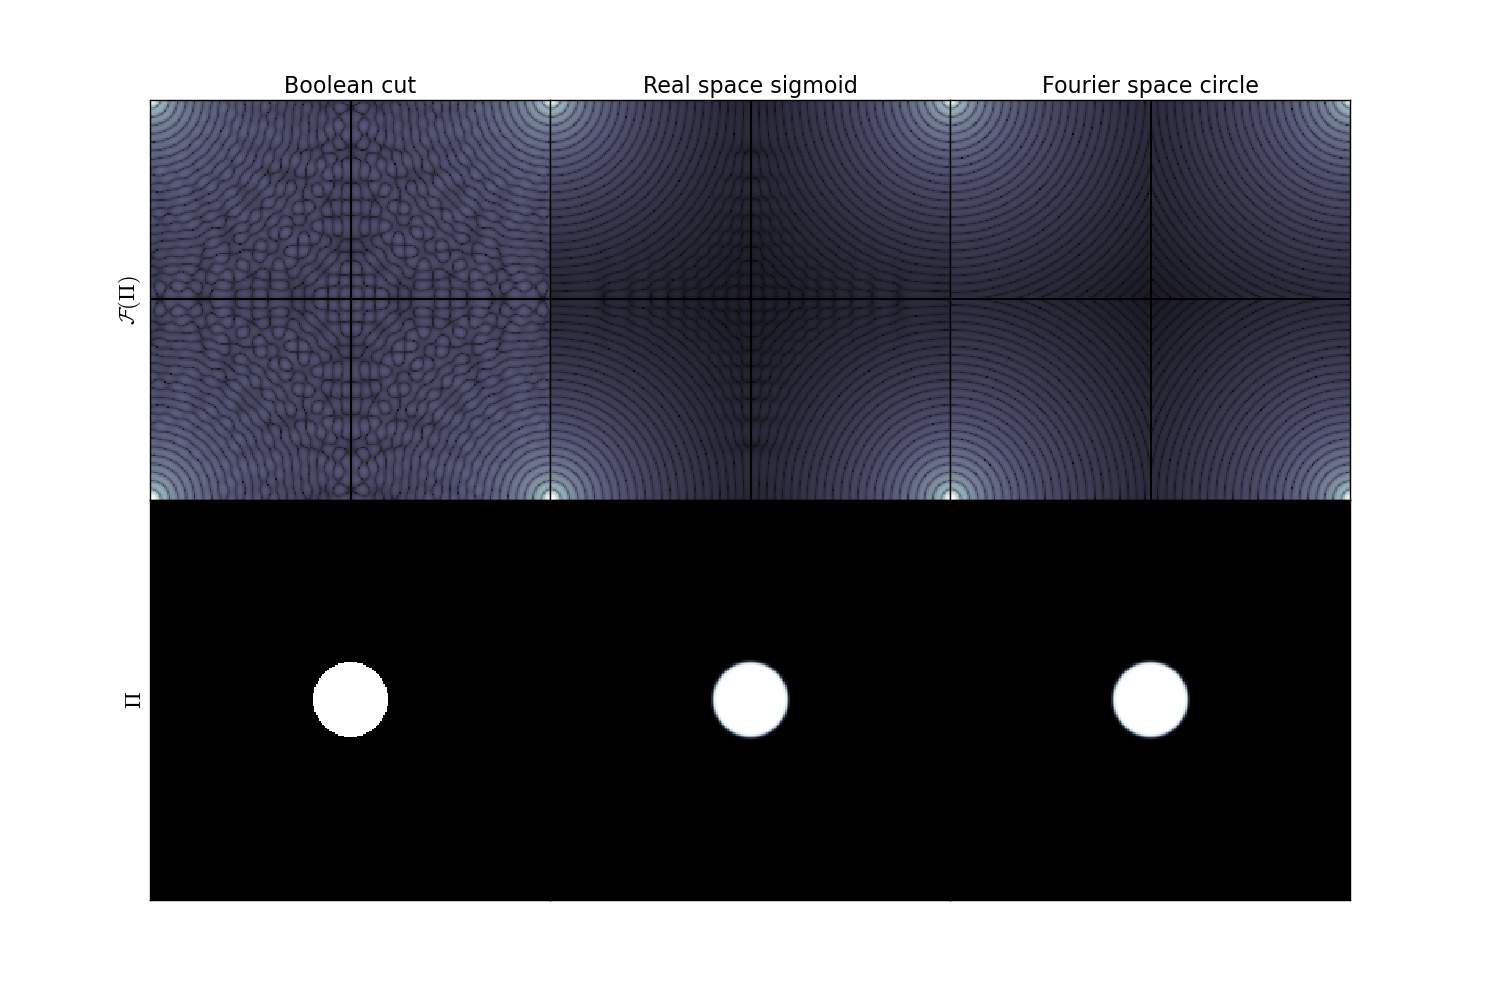
\includegraphics[width=0.95\columnwidth]{figs/sphere_generation_comparison.png}

    \caption{A comparison of different methods to create an image of a sphere.
        These methods are (left) making a boolean cut as a function of the
        distance from the center (middle) using a sigmoidal function $\Pi(r) =
        (1 + e^{-\alpha r_0}) / (1 + e^{\alpha (r - r_0)})$ and (right) using the Fourier shape
    generation described in this section.}

    \label{fig:sphere_generation_comparison}
\end{figure}



\subsection{CCDs have noise}

We generate our true image, we must also include intrinsic shot noise.
Theoretically, this type of noise is the only part of the confocal image
that we will not be able to reconstruct in any way.  In particular, it
will be the noise distribution that we use to create our likelihood function
meaning given a hyperparameter which describes its distribution.

To make this noise, at the last step of the image generation process, we
add a random field to the CCD,

\begin{equation}
    I(\vec{x}) = I(\vec{x}) + N(\vec{x}, \mu, \sigma)
\end{equation}

where $\langle N(\vec{x}^a_i, \mu, \sigma) N(\vec{x}^b_j, \mu, \sigma)\rangle =
\delta^{ab} \delta_{ij}$ and $\sigma$ determines the standard deviation of that
noise.

\bibliography{references}

\end{document}
